\documentclass{article}

\usepackage{url}
\usepackage{enumitem}

\RequirePackage[colorlinks]{hyperref}

%%% From https://tex.stackexchange.com/questions/447399/how-to-create-eisenhower-matrix-notepad-in-latex
\usepackage{tikz,amssymb}
\usetikzlibrary{shapes.multipart,positioning,fit,backgrounds}
\definecolor{mgreen}{RGB}{22,171,53}
\definecolor{mblue}{RGB}{22,101,171}

\newcommand{\EisenBlock}[5][]{
  \node [rectangle split,rectangle split parts=8,fill=white,
  text width=5cm,align=left,text=#2,draw,rounded corners,draw=#2,
  #1] 
  (multi-#3)
 {\strut$\Box$ \EntryOne\nodepart{two}\strut$\Box$ \EntryTwo
 \nodepart{three}\strut$\Box$ \EntryThree\nodepart{four}\strut$\Box$ \EntryFour
 \nodepart{five}\strut$\Box$ \EntryFive\nodepart{six}\strut$\Box$ \EntrySix
 \nodepart{seven}\strut$\Box$ \EntrySeven\nodepart{eight}\strut$\Box$ \EntryEight};
 \node[left=1pt of multi-#3.south west,anchor=south west,rotate=90,text=white] 
 (label-#3) {#4};
 \begin{scope}[on background layer]
 \node[fit=(multi-#3) (label-#3),fill=#2,rounded corners,
 label={[text=#2,anchor=south west,font=\bfseries]above left:#5}] (fit-#3){};
 \end{scope}
 \ClearEntries
}

\newcommand{\SetEntries}[8]{
\def\EntryOne{#1}
\def\EntryTwo{#2}
\def\EntryThree{#3}
\def\EntryFour{#4}
\def\EntryFive{#5}
\def\EntrySix{#6}
\def\EntrySeven{#7}
\def\EntryEight{#8}}
\newcommand{\ClearEntries}
{\SetEntries{\empty}{\empty}{\empty}{\empty}{\empty}{\empty}{\empty}{\empty}}
\ClearEntries


\title{All Things Authentication}
\date{\today}
\author{Dave Doolin}

\begin{document}
\maketitle
\tableofcontents

\section{Introduction}

An authentication bible collects up information on how authentication works,
in one easy to read reference work. While my usual, initial and default habit,
is exhaustive exploration, that never gets to any sort of completion. For this
document, structuring the work in terms of Objective and Key Results (OKRs),
which will provide both a roadmap, and a notion of when it's complete.

\paragraph{Objective} Create an In-depth Primer on Deployed Authentication

% TODO: Clean up the formatting here:
% * no indentation for "Key Result"
% * small indentation for the enum list following.
Key Results:

% http://mirrors.ibiblio.org/CTAN/macros/latex/contrib/enumitem/enumitem.pdf
% https://ctan.org/pkg/enumitem?lang=en
\begin{enumerate}[label=KR\arabic*]
  \item Description and example of Basic authentication.
  \item Description and example of JSON Web Token.
  \item Description and example of Devise usage.
  \item Description and example of Google Auth and SAML for SSO.
\end{enumerate}

% TODO: define in detail what "Description" and "Example" mean

\subsection{HTTP Sessions}

Placeholder for discussion of HTTP Sessions. duckduckgo seems
to have some good search results.

\section{Basic Auth}

From \href{https://en.wikipedia.org/wiki/Basic_access_authentication}{%
  HTTP Basic Access Authentication on Wikipedia}, is a method for an HTTP
user agent to provide a user and password when making a request. The request
contains a header field in the form \texttt{Authorization: Basic
 <credentials>}. Credentials are in the form \texttt{username:password} encoded in
Base64, that is, the \texttt{username} and \texttt{password} are separated by a colon
and Base64 encoded.

Basic Auth (BA) is the simplest technique for enforcing access control to
web resources as it does not require cookies, session identifiers, or
login pages. API call authentication over HTTPS is a common use case.

Some notes:
\begin{itemize}
  \item \href{https://tools.ietf.org/html/rfc7617}{%
      RFC 7617 The 'Basic' HTTP Authentication Scheme} is the
    canonical reference.
  \item MacOs has the \texttt{base64} available for the command line. Utilities
    exist in Ruby, Python, etc. for managing base64 encoding.
  \item \href{https://api.rubyonrails.org/classes/ActionController/HttpAuthentication/Basic.html}{%
      Basic Auth is part of Rails}, hence available to every Rails application.
\end{itemize}

\subsection{Basic Auth in Rails}

The key is using \href{https://github.com/rails/rails/blob/master/actionpack/lib/action_controller/metal/http_authentication.rb}{%
Rails' built in Basic Auth system}.

% TODO: Explain how the SecurePassword is used in a service.
The key is the \texttt{authenticate} metaprogramming
\href{https://github.com/rails/rails/blob/master/activemodel/lib/active_model/secure_password.rb#L119}{%
  defined in ActiveModel::SecurePassword}.

Here is \href{https://www.youtube.com/watch?v=O1sgFzn_Pgk}{%
a great video on macros in Ruby}; ruby macros are used extensively in Rails.

\subsection{Exercises}

\begin{itemize}
  \item Run the following from the command line: \texttt{%
      echo "username:password" | base64}. What is returned?
    I get \texttt{dXNlcm5hbWU6cGFzc3dvcmQK}.
  \item Examine the HTTP request headers for a service using Basic Auth
    to see how the header looks.
  \item Find some source code using Basic Auth and understand how
    it's implemented in that code. If you can't find anything, write
    a simple open source example for yourself.
\end{itemize}



\section{JWT}

JSON Web Token (JWT) is a URL-safe means for representing
claims in JSON format to be transferred between two parties.
Tokens are signed with either a private secret, or a public/private
key pair.

% TODO: add a quad diagram of encryption and signing options
% TODO: create a quad diagram macro for general use

Some notes:

\begin{itemize}
  \item \href{https://en.wikipedia.org/wiki/JSON_Web_Token}{%
     JSON Web Token on Wikipedia}
  \item \href{https://tools.ietf.org/html/rfc7519}{%
     RFC 7519 JSON Web Token (JWT)}
 \item JWT may used to implement SSO.
 \item JWTs can be signed using a secret (with HMAC algorithm) or a
   public/private key pair using RSA.
 \item \href{https://auth0.com/learn/json-web-tokens/}{%
Get Started with JSON Web Tokens} from Auth0.
  \item In Ruby, the order of elements in a hash matters when signing, because the
        gets turned into a string.
\end{itemize}

TODO: Search for how Rails can work with JWT, either as a ID server,
or as a client (or both?).

TODO: Investigate ordering in simple Javascript objects corresponding to Ruby hashes.

TODO: Split the jwt example scripts into 3 parts.

\subsection{An example authentication server}

Three parts:

\begin{enumerate}
  \item Client 1: logs into Auth server, retrieves token, queries Service 1.
        Client 1 probably only needs to store whole token, without any processing of token.
  \item Service 1: accepts token from Client 1, returns data.
  \item Auth server: accepts login credentials from Client 1, returns token.
\end{enumerate}


% TODO: This picture needs to be turned into a quad which explains how JWE and JWS
% work within the JWT framework.
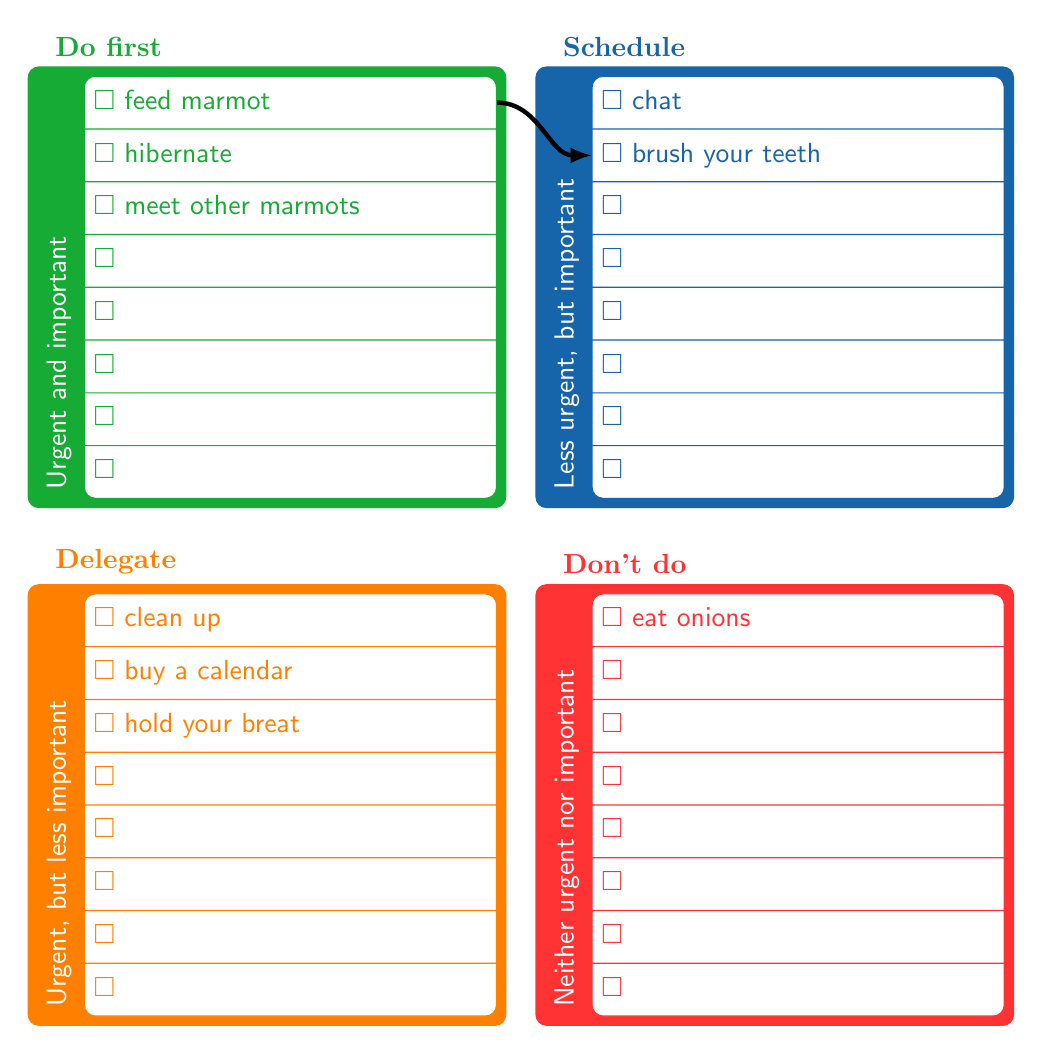
\begin{tikzpicture}[font=\sffamily]
  \SetEntries{feed marmot}{hibernate}{meet other marmots}{}{}{}{}{}
  \EisenBlock{mgreen}{tl}{Urgent and important}{Do first}
  \SetEntries{chat}{brush your teeth}{}{}{}{}{}{}
  \EisenBlock[right=1.2cm of multi-tl]{mblue}{tr}{Less urgent, but
  important}{Schedule}
  \SetEntries{clean up}{buy a calendar}{hold your breat}{}{}{}{}{}
  \EisenBlock[below=1.2cm of multi-tl]{orange}{bl}{Urgent, but
  less important}{Delegate}
  \SetEntries{eat onions}{}{}{}{}{}{}{}
  \EisenBlock[right=1.2cm of multi-bl]{red!80}{br}{Neither urgent nor
  important}{Don't do}
  \draw[ultra thick,-latex] (multi-tl.one east) to[out=0,in=180]
  (multi-tr.two west);
\end{tikzpicture}
\section{HTTP Digest}

HTTP Digest can be used when the client is a web browser. From Wikipedia,
digest authentication is an application of MD5 cryptographic hashing with usage
of nonce values to prevent replay attacks.

From \href{https://en.wikipedia.org/wiki/Digest_access_authentication}{HTTP Digest on Wikipedia}.

\begin{itemize}
  \item \href{https://tools.ietf.org/html/rfc7616}{%
      RFC 7616 HTTP Digest Access Authentication}
\end{itemize}



\section{HTTP Token}




\section{Form-based authentication}
\section{HMAC}
\section{OAuth}
\section{OAuth2}
\section{SAML}
\section{OpenID}
\section{BrowserID}

\appendix

\section{Useful links}

\begin{itemize}
  \item \href{https://blog.restcase.com/restful-api-authentication-basics/}{%
      RESTful API Authentication Basics}
\end{itemize}

\section{Glossary}

\paragraph{base64url} \href{https://en.wikipedia.org/wiki/Base64#URL_applications}{%
  Base64Url} as described in \href{https://tools.ietf.org/html/rfc4648}{%
    RFC 4648 The Base16, Base32, and Base64 Data Encoding}

\section{Source code}

\section{TODO}

\begin{itemize}
  \item Explain the difference in JWT between using a private secret and a
    public/private key pair.
  \item Read through source of \texttt{http\_authentication} to understand how
    the methods are implemented.
  \item Add HTTP Basic Auth to Anki deck, including all relevant material from
    RFC 7617.
  \item Can Rails Token Auth accept JWT?
  \item Refactor rack Basic Auth example.
\end{itemize}

\end{document}
